\section{Guardians and kindergarten teacher}
The kindergarten teacher is a very important person in the life of an autistic child. The kindergarten teacher is the person who helps and guards the autistic child. The kindergarten teacher and the child develop a special relationship to each other. The kindergarten teacher follows the child in a some of its everyday life and in the case of Birken, the kindergarten teachers follows each child individually in 17 hours each week. Birken is a kindergarten for special-needs children which is located at Vodskov in Northern Denmark Region.

Employees/pedagogues from Birken have been included in the projected by the groups in the multi-project and in this project. Our contact from Birken Christine Niss-Henriksen have been included in this project because of her knowledge about children with autism and technological knowledge who then would be able to help come up with ideas and opinions about our program and finally test the final program.  

\subsection{PACT}
%ulriks kommentar:"Taler I om den nuv�rende situation eller om systemet her?" bliver allerede sagt her
After the first interview with Christine, which is in \vref{first_interview_birken}, we decided to include a digitized version of their contact book in our project. %The contact book is primary a communication tool that the kindergarten teachers and the parents use to write messages to each other concerning the child and this book is then transported with the child.  
A PACT analysis was made on the current application of the contact book based from the information gathered from the interview, see PACT model in \vref{fig:PACT}. PACT is an acronym for People, Activities, Contexts and Technologies, and this analysis is general use for understanding how people undertake activities in a certain context often using some form of technology. The individual parameters are described in their respective headers in our PACT. 

\begin{figure}
	\centering
		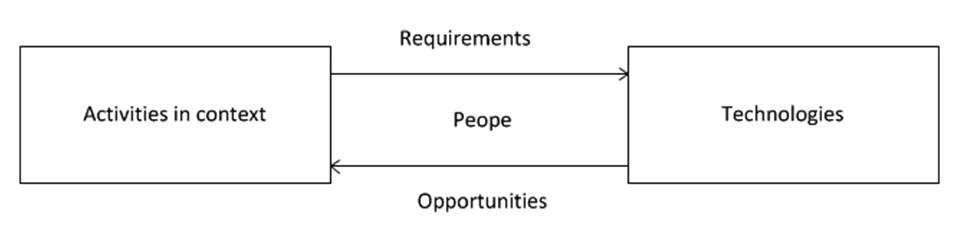
\includegraphics[width=0.70\textwidth]{img/PACT.png}
	\caption{PACT model}
	\label{fig:PACT}
\end{figure}



\subsubsection{People - the kindergarten teacher}
Christine is in her thirties and is a fully educated pedagogue. Beyond this she has taken several degrees and courses focusing on the needs of children with mental handicaps, all resulting in her now working at Birken.

She takes care of a select few children of those attached to the kindergarten, an activity that requires almost constant supervision while they are present. Christine and her colleagues yearn for solutions that can ease and improve their daily work, particularly within the domains of communication with the children and their parents. Very notably, the time required to add a picture to an entry in the child's contact book is so severe that she cannot do it very often, a hindrance that bothers her. She would very much like to be able to attach an image to the book every day to improve the dialogue between child and parent.

\subsubsection{Activities}
\begin{itemize}
	\item Each day an entry is written in the contact book of every child, detailing the highlights of the day. It may be a single sentence or a paragraph with a picture of the child engaging in an activity. This is done by the guardians at the kindergarten, but entries may be commented or entered a new by parents with any important thoughts.
	\item If a picture is to be added, first the picture is taken with a digital camera, imported into a desktop computer, then cropped, resized or rotated as necessary. Finally, the image is printed onto paper, cut out and glued into the contact book.
	\item Child and parent will sit down with the book, using the image in the book (if present) as a starting point for dialogue about the day, continuing through available pictograms.
\end{itemize}

\subsubsection{Contexts}
There are three contexts based on the three activities, two of them sufficiently similar to be written as one.
\begin{itemize}
	\item When compiling an entry in the contact book, the kindergarten teacher or guardian will sit by themselves, the child occupied either with their own devices or the supervision of someone else. 
	\item When discussing the entry in the book, however, child and parent are together.
\end{itemize}

\subsubsection{Technology}
Currently, two hardware technologies are in play: A digital camera, and a personal computer.
An image manipulation suite is used to edit the photographs. Possibly, this is a Windows pre-installed application like MS Paint.

\subsubsection{Conclusion}
Even at a glance, several possible improvements can be suggested that make use of IT. Central are the notions of digitizing the contact book and easing the creating of images by using a mobile device with image manipulation software capable of the actions usually necessary.